%%%%%%%%%%%%%%%%%%%%%%%%%%%%%%%%%%%%%%%%%
% Beamer Presentation
% LaTeX Template
% Version 1.0 (10/11/12)
%
% This template has been downloaded from:
% http://www.LaTeXTemplates.com
%
% License:
% CC BY-NC-SA 3.0 (http://creativecommons.org/licenses/by-nc-sa/3.0/)
%
%%%%%%%%%%%%%%%%%%%%%%%%%%%%%%%%%%%%%%%%%

%----------------------------------------------------------------------------------------
%	PACKAGES AND THEMEShttps://www.overleaf.com/project/5dbfadb88b2560000102ab44
%----------------------------------------------------------------------------------------

\documentclass{beamer}

\mode<presentation> {

% The Beamer class comes with a number of default slide themes
% which change the colors and layouts of slides. Below this is a list
% of all the themes, uncomment each in turn to see what they look like.

%\usetheme{default}
\usetheme{AnnArbor}
%\usetheme{Antibes}
%\usetheme{Bergen}
%\usetheme{Berkeley}
%\usetheme{Berlin}
%\usetheme{CambridgeUS}
%\usetheme{Copenhagen}
%\usetheme{Darmstadt}
%\usetheme{Dresden}
%\usetheme{Frankfurt}
%\usetheme{Goettingen}
%\usetheme{Hannover}
%\usetheme{Ilmenau}
%\usetheme{JuanLesPins}
%\usetheme{Luebeck}
%\usetheme{Madrid}
%\usetheme{Malmoe}
%\usetheme{Marburg}
%\usetheme{Montpellier}
%\usetheme{PaloAlto}
%\usetheme{Pittsburgh}
%\usetheme{Rochester}
%\usetheme{Singapore}
%\usetheme{Szeged}
%\usetheme{Warsaw}

% As well as themes, the Beamer class has a number of color themes
% for any slide theme. Uncomment each of these in turn to see how it
% changes the colors of your current slide theme.

%\usecolortheme{albatross}
%\usecolortheme{beaver}
%\usecolortheme{beetle}
%\usecolortheme{crane}
%\usecolortheme{dolphin}
%\usecolortheme{dove}
%\usecolortheme{fly}
%\usecolortheme{lily}
%\usecolortheme{orchid}
%\usecolortheme{rose}
%\usecolortheme{seagull}
%\usecolortheme{seahorse}
%\usecolortheme{whale}


%\usetheme{Boadilla}
\usecolortheme{wolverine}

%\setbeamertemplate{footline} % To remove the footer line in all slides uncomment this line
\setbeamertemplate{footline}[page number] % To replace the footer line in all slides with a simple slide count uncomment this line

\setbeamertemplate{navigation symbols}{} % To remove the navigation symbols from the bottom of all slides uncomment this line
}

\setbeamertemplate{bibliography item}{\insertbiblabel}


\usepackage{graphicx} % Allows including images
\usepackage{booktabs} % Allows the use of \toprule, \midrule and \bottomrule in tables
%\usepackage {tikz}
\usepackage{tkz-graph}
\usepackage{bibentry}


\usepackage[
backend=biber,
style=numeric,
sorting=ynt
]{biblatex}
 
\documentclass[xcolor=table]{beamer} 

\bibliography{bibfile}

\graphicspath{ {images/} }

\GraphInit[vstyle = Shade]
\tikzset{
  LabelStyle/.style = { rectangle, rounded corners, draw,
                        minimum width = 2em, fill = yellow!50,
                        text = red, font = \bfseries },
  VertexStyle/.append style = { inner sep=5pt,
                                font = \normalsize\bfseries},
  EdgeStyle/.append style = {->, bend left} }
\usetikzlibrary {positioning}
%\usepackage {xcolor}
\definecolor {processblue}{cmyk}{0.96,0,0,0}

% show sections only
\setcounter{tocdepth}{1}
% show subsections
%\setcounter{tocdepth}{2}
% show subsubsections
%\setcounter{tocdepth}{3}
\AtBeginSection[]
{
    \begin{frame}
        \frametitle{Table of Contents}
        \tableofcontents[currentsection]
    \end{frame}
}

%\AtBeginSubsection[]
%{
%    \begin{frame}
%        \frametitle{Table of Contents}
%        \tableofcontents[currentsection,currentsubsection]
%    \end{frame}
%}

%----------------------------------------------------------------------------------------
%	TITLE PAGE
%----------------------------------------------------------------------------------------

\title[caDDS]{caDDS: Community Assisted Distributed Database for Sequences} 

%%%%%%%%%%%%%%%%%%%%%%%%%%% INFO %%%%%%%%%%%%%%%%%%%%%%%%%%%%%%%%%%%%%%%%%%%%%%%%%

\author{Azcarraga, Araya} % Your name
\institute[Department of Computer Science, University of the Philippine - Diliman] % Your institution as it will appear on the bottom of every slide, may be shorthand to save space
{
University of the Philippine - Diliman\\ % Your institution for the title page
\medskip
}
\date{\today} % Date, can be changed to a custom date


%----------------------------------------------------------------------------------------
%	PRESENTATION SLIDES
%----------------------------------------------------------------------------------------


\begin{document}

%%%%%%%%%%%%%%%%%%%%%%%%%%%%% TITLE %%%%%%%%%%%%%%%%%%%%%%%%%%%%%%%%%%%%%%%%%%%%%%
\begin{frame}
\titlepage % Print the title page as the first slide
\end{frame}


%%%%%%%%%%%%%%%%%%%%%%%%%%%%% OVERVIEW %%%%%%%%%%%%%%%%%%%%%%%%%%%%%%%%%%%%%%%%%%%%%%
\begin{frame}
\frametitle{Overview} % Table of contents slide, comment this block out to remove it
\tableofcontents % Throughout your presentation, if you choose to use \section{} and \subsection{} commands, these will automatically be printed on this slide as an overview of your presentation
\end{frame}

%%%%%%%%%%%%%%%%%%%%%%%%%%%%% INTRO + RRL %%%%%%%%%%%%%%%%%%%%%%%%%%%%%%%%%%%%%%%%%%%%%%
\begin{frame}{Abstract}
  Genomic data the past few years have grown exponentially with the technology barely keeping up. The problem faced by genome researchers is the large data set and difficulty transferring the files. Previous distributed databases are either not meant for genomic data, or difficult to replicate. This paper lays the groundwork for a distributed database that is designed to easily scale to accommodate bigger storage, and also reduces the data speed bottleneck faced by centralized databases. The proposed system has a master node and data nodes. Data nodes should theoretically increase data transfer speeds even as the number of users increase. (to be updated based on conclusion) While current databases(e.g. NCBI) have more data, more users, and a live platform. The proposed system is aimed towards a smaller community, with more frequent and localized data, which the data storage can easily be expanded as the need arises. A recommendation is to implement the system and make the code public for the use of other communities.
\end{frame}
\section{Introduction}
\subsection{Genomic Concepts}

\begin{frame}{Human DNA Length}
    \centering
    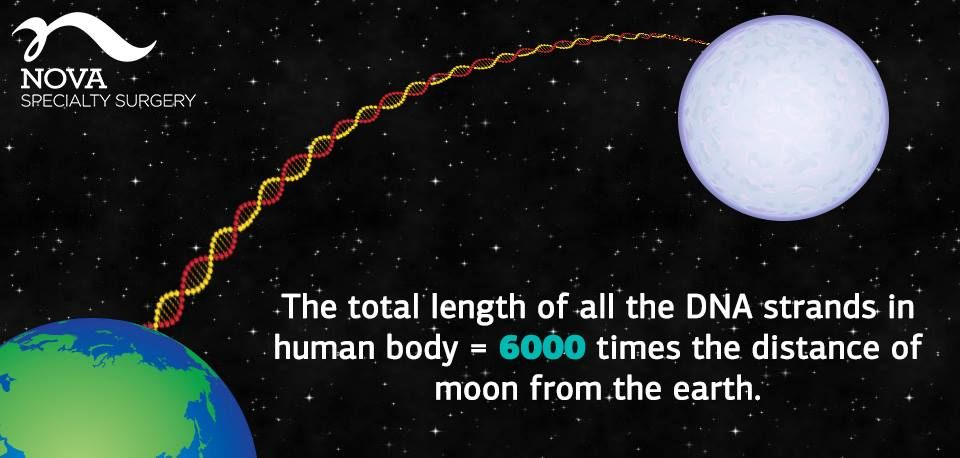
\includegraphics[scale=0.3]{dna-length.jpg}
\end{frame}

\begin{frame}{Genes}
  \begin{itemize}   
    \item all organisms have genes
    \item Genes are made of a certain molecular structure called DNA which correspond to information denoted by: A,G,C,T
    \item Genes are instructions and blueprints for life
  \end{itemize}
\centering
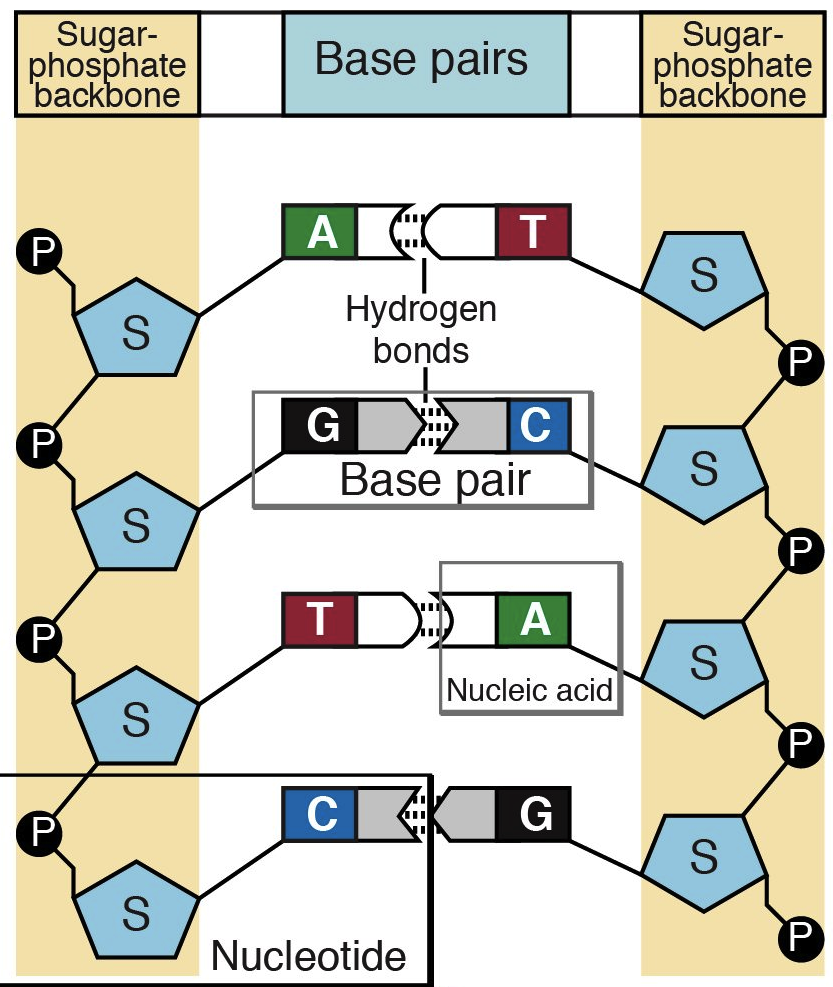
\includegraphics[scale=0.1]{gene-base-pair.png}
\end{frame}

\begin{frame}{Human Genes}
  \begin{itemize}   
    \item There is a lot of information in one human cell
    \item One human cell's entire genes laid out is 2 meters in length \cite{ency_sci_tech} and has $3.2x10^9$ base pairs \cite{introgenomics}
    \item Human body has a lot of information, that when laid out spans the earth to the moon six thousand times
\end{itemize}
\end{frame}


\begin{frame}{Genomics}
  \begin{block} {\textbf{Definition of Genomics}}
    Genomics is the study of all of a person's genes (the genome), including interactions of those genes with each other and with the person's environment. \cite{genomics-definition}
  \end{block}
  \begin{itemize}   
    \item \textbf{Genomics}: study of whole sets of genes and their interactions \cite{campbell}
    \item More complex organisms have more complex genes (many parts and interactions)
    \item Studying these complex organisms needs a lot of storage
    \item The current online portal mainly used to study this is NCBI \cite{campbell}
  \end{itemize}
\end{frame}

\begin{frame}{Sequencing}
  \begin{itemize}   
    \item Reading genes from cells is sequencing
    \item Replications (coverage) \& Fragmentation of DNA is necessary to read
    \item Every read stores the many fragments
    \item Each sequence read is redundant and uses a lot of space
  \end{itemize}
  \centering
  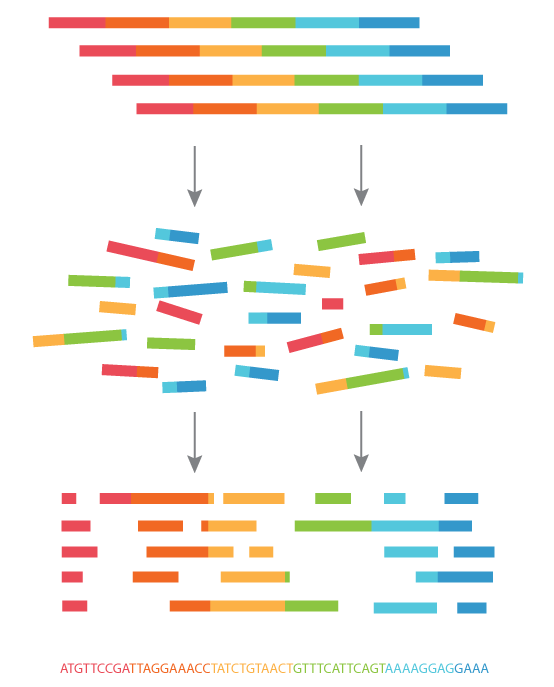
\includegraphics[scale=0.2]{sequencing.png}
\end{frame}

\begin{frame}{Human Genome Project Successes}
  \begin{itemize}   
    \item 2 years after, the project led to a whole genome project for chimpanzees (human's closest relative) \cite{campbell}
    \item These led to many whole genome analysis of organisms (around 4,300 in 2013) \cite{campbell}
    \item Growing amount of research and data from genome research.
  \end{itemize}
\end{frame}

\begin{frame}{Human Genome Project}
  \begin{itemize}   
    \item Finished in 2003, project wanted to read the entire human genome
    \item Didn't have the mature tools at the time
    \item Big cost, many institutions, 10 years \cite{introgenomics}
  \end{itemize}
\end{frame}

\begin{frame}{Next Generation Sequencing}
  \begin{itemize}
    \item original sequencing for HGP took ten years, now (2019) one laboratory can do 10,000 a day (36.5 million times faster)  \cite[p.~19]{introgenomics}   
    \item New sequencing technology to read faster and cheaper
    \item Faster reads corresponds to more data
  \end{itemize}
\end{frame}

\begin{frame}{Human genome cost over time}
Graph of human genome cost over time \cite{genomics-cost} \\
\centering
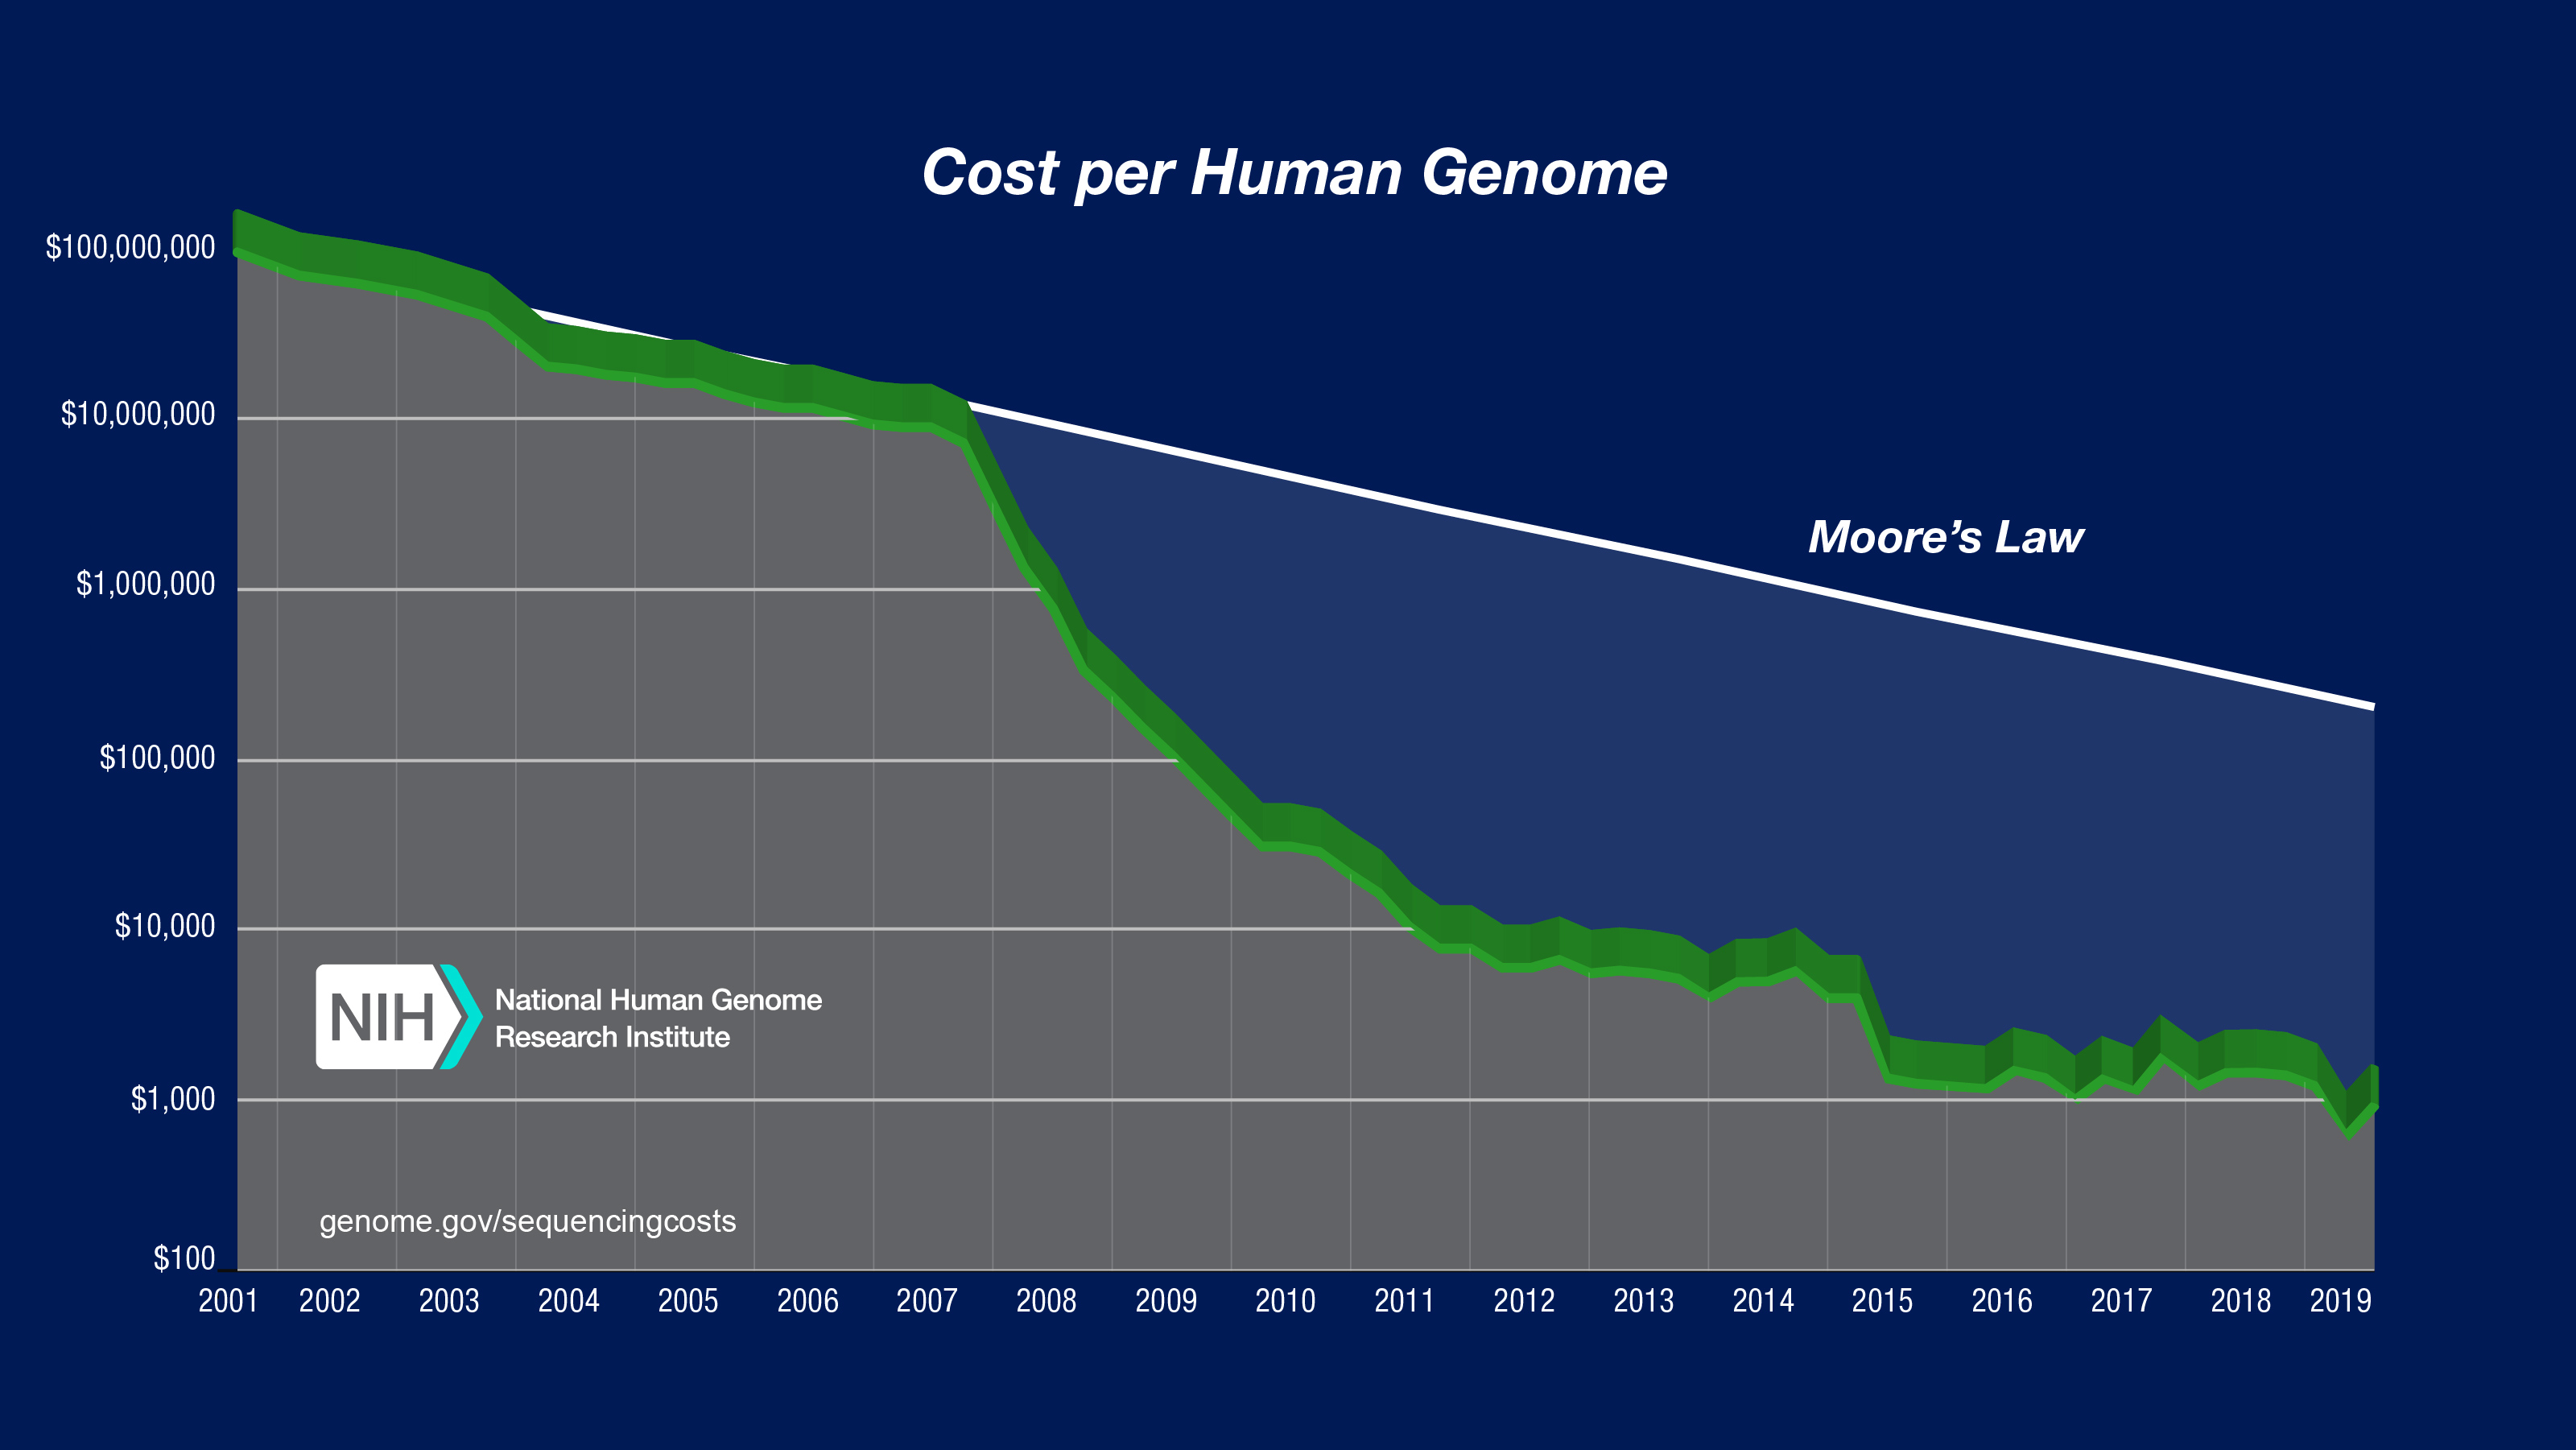
\includegraphics[scale=0.3]{human-gen-cost.jpg}
\end{frame}
    
\begin{frame}{Sequence data cost over time}
Graph of a megabase sequence cost over time \cite{genomics-cost}
\begin{itemize}
    \item Megabase means one million bases
\end{itemize}
\centering
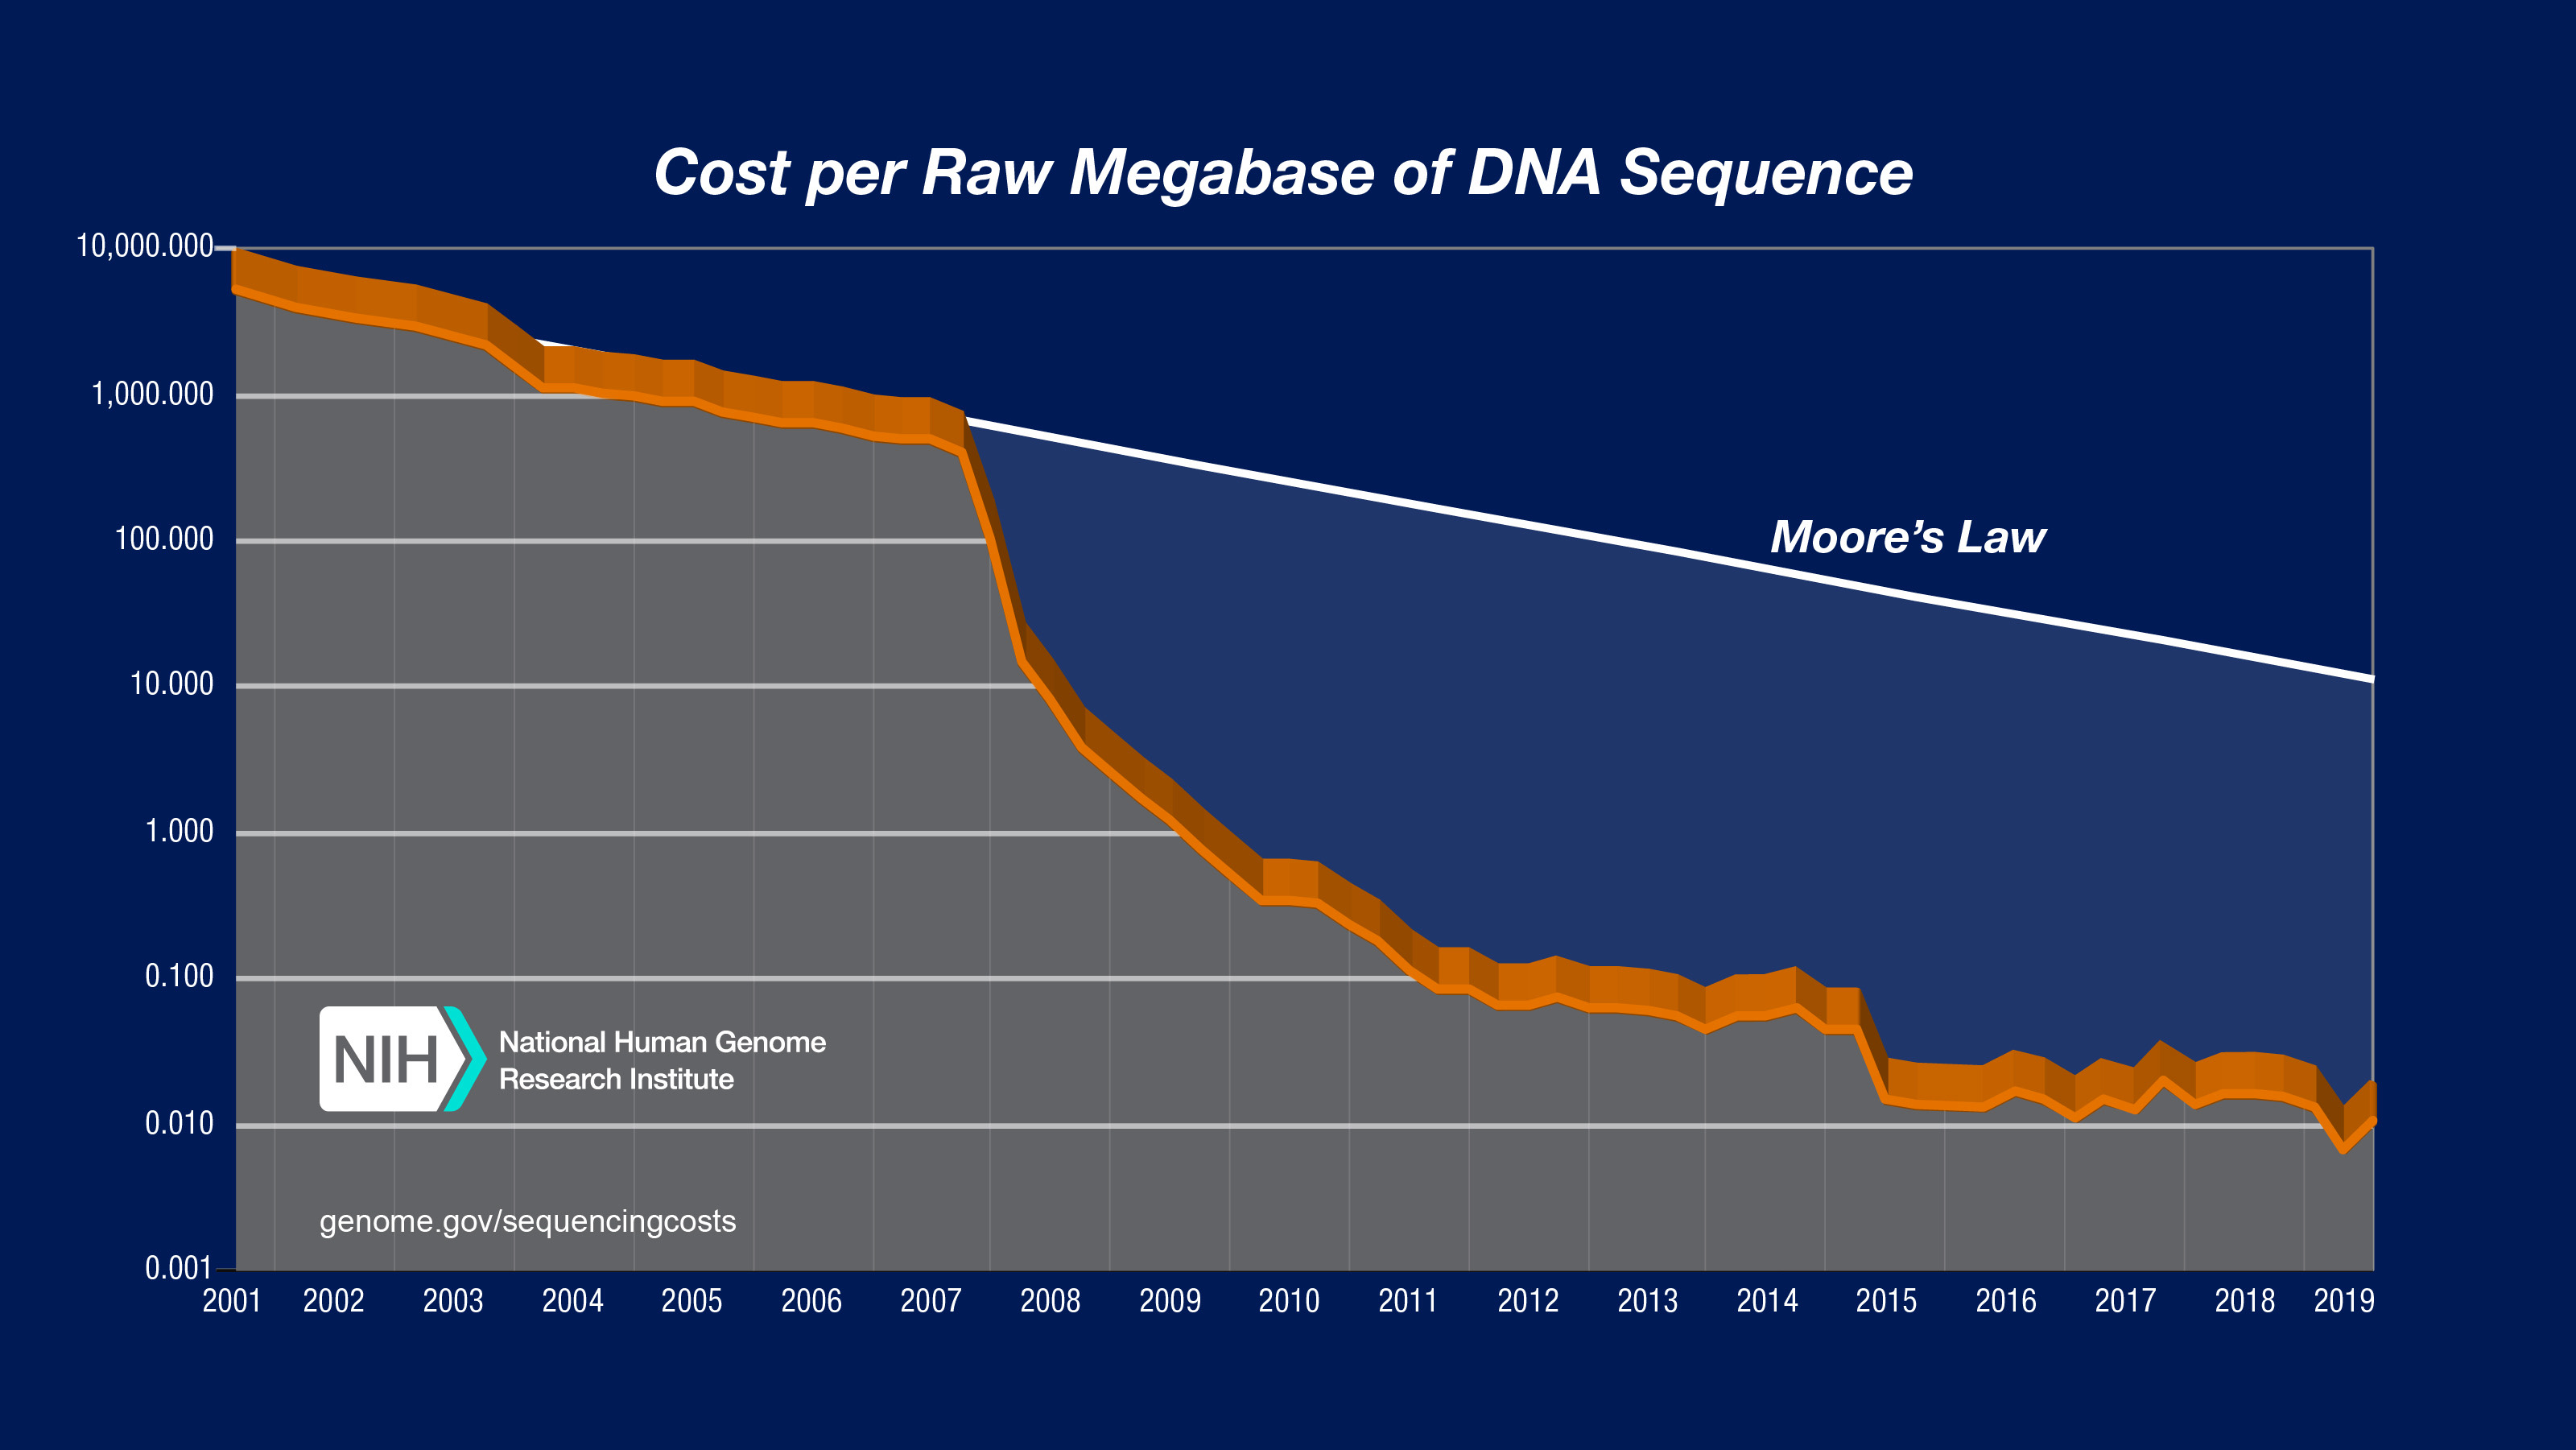
\includegraphics[scale=0.1]{seq-cost.jpeg}
\end{frame}

\begin{frame}{NGS vs Hard Disk Storage}
        Computational sense, there is a need to store, upload, and retrieve sequence files that are growing larger. 
        \begin{itemize}
        \item Slope of orange line (NGS) is larger than slope of yellow line (pre-NGS)
        \item Hard disk storage (blue) graph is greater than yellow (pre-NGS) but is now less than orange (NGS)
        \end{itemize}
        \centering
            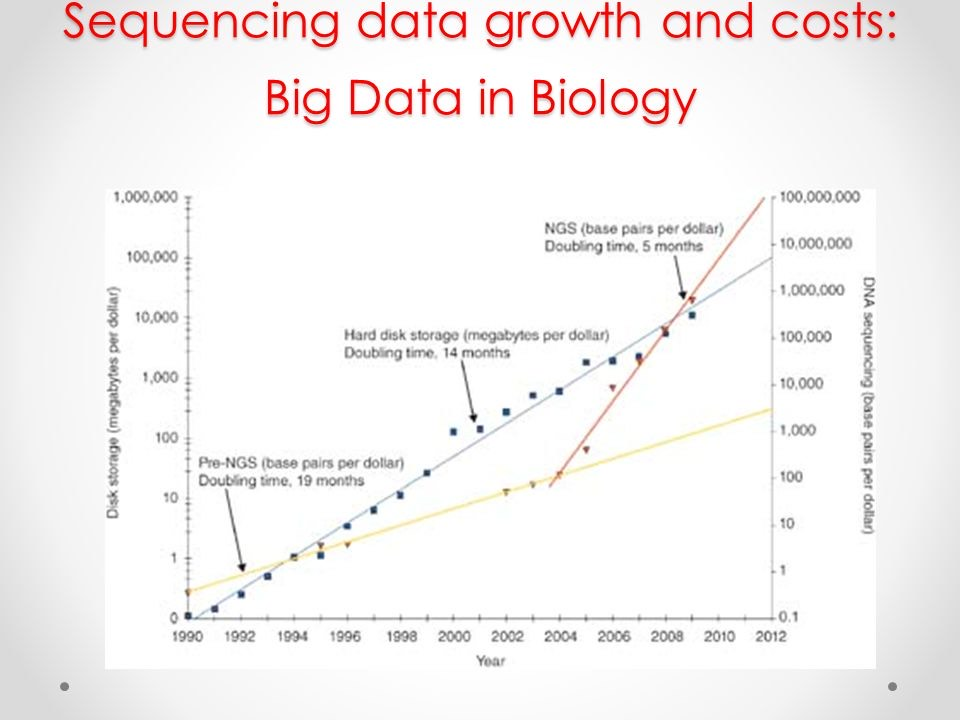
\includegraphics[scale=0.2]{seq-data.jpeg}
\end{frame}

\begin{frame}{Moore's Law}
  \begin{block}{\textbf{Moore's law}} 
    states that the number of transistors on a chip doubles every two years.\cite{kurose}
  \end{block}
  \begin{itemize}   
    \item Prediction of the speed new technology (faster processing power and better storage) is developed
    \item But moore's law is too slow for the speed of genomic data increase
    \item
  \end{itemize}
\end{frame}

\begin{frame}{Growing problem of storage}
  \begin{itemize}   
    \item Each read\cite{seqtorr} has 60x coverage, around 200gb each
    \item NGS, More genomic researches, more files needed to be saved and transferred
  \end{itemize}
\end{frame}

\subsection{Data Storage Concepts}
\begin{frame}{Database}
  \begin{itemize}   
    \item store data with tech
  \end{itemize}
\end{frame}
  \begin{frame}{Data Storage}
        A \textbf{database} (\textbf{DBMS}, Database Management System) is defined by 
        \begin{block} {\textbf{Definition}}

        DBMS contains information about a particular enterprise
        \begin{itemize}
            \item Collection of interrelated data
            \item Set of programs to access the data 
            \item An environment that is both convenient and efficient to use
        \end{itemize}
        \cite{Silberschatz2010}
        \end{block}
    \end{frame}
    
    \subsubsection{Database Principles}
    \begin{frame}{Database Principles}
        \begin{itemize}
            \item \textbf{Principles} to remember when creating a database (CAP). Idea is that only 2 of the three can be focused on. \cite[Ch.~19]{Silberschatz2010}
            \begin{itemize}
                \item \textbf{Consistency}
                \begin{itemize}
                    \item Update one part, will all other (replicated) parts be updated quickly as well
                    \item Data is accurate and copied faithfully
                \end{itemize}
                \item \textbf{Accessibility}
                \begin{itemize}
                    \item How easy it is to access data
                    \item API protocols
                \end{itemize}
                \item  \textbf{Partition Tolerance}
                \begin{itemize}
                    \item If one portion breaks, the other portions are still usable
                    \centering 
                    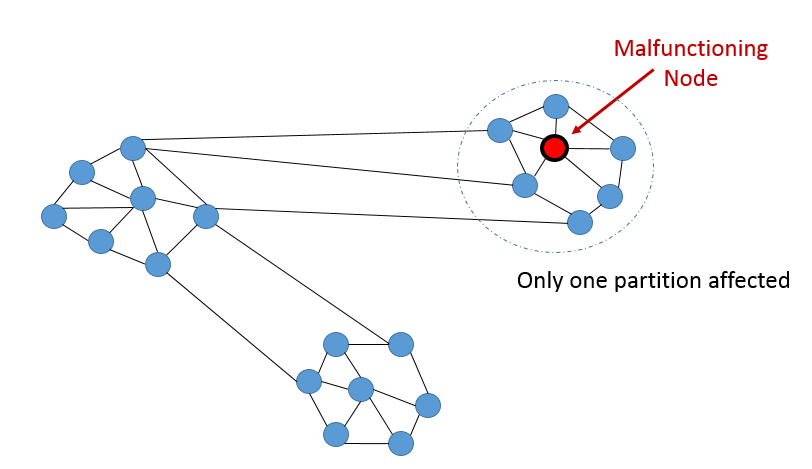
\includegraphics[scale=0.2]{partition_tolerance.png}
                    \end{itemize} 
             \end{itemize}
        \end{itemize}
    \end{frame}
  \begin{frame}{Normal: NCBI}
        \begin{itemize}
            \item NCBI has a large collection of genomic datasets in its website, which can be searched and downloaded.
        \end{itemize}
    \end{frame}
    \begin{frame}{Normal: NCBI}
        \begin{itemize}
            \item Search page https://www.ncbi.nlm.nih.gov/nucleotide
            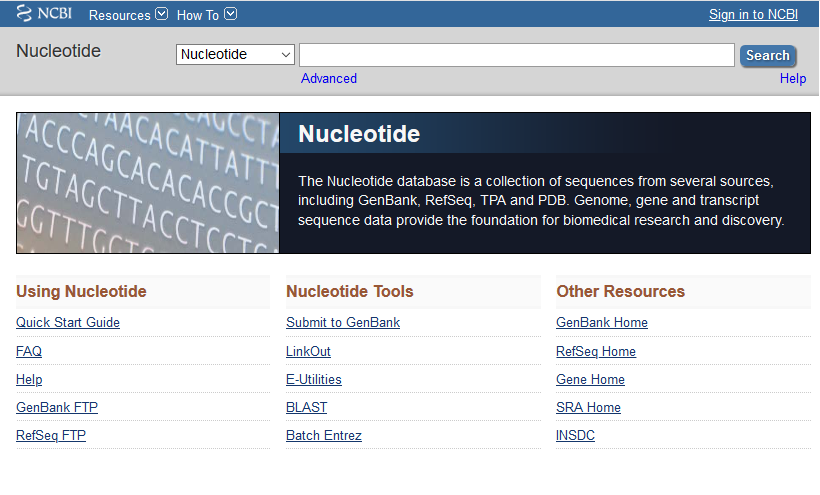
\includegraphics[scale=0.5]{ncbi1.png}
        \end{itemize}
    \end{frame}
    \begin{frame}{Normal: NCBI}
        \begin{itemize}
            \item List of results
            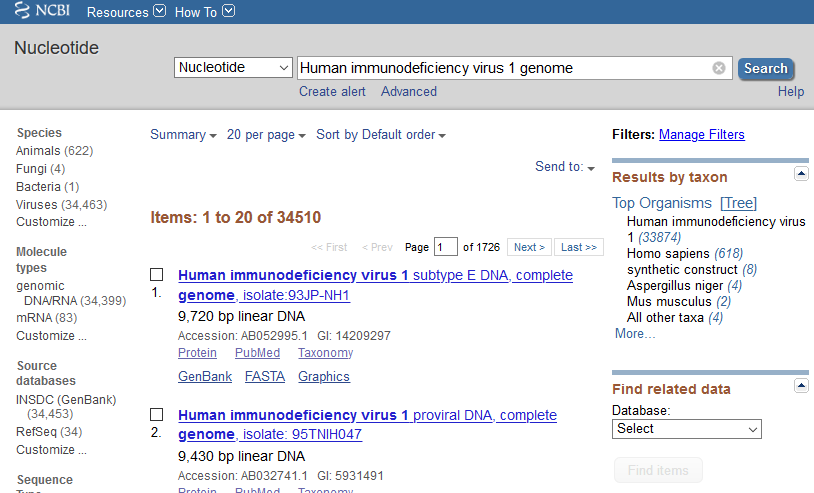
\includegraphics[scale=0.5]{ncbi2.png}
        \end{itemize}
    \end{frame}
    \begin{frame}{Normal: NCBI}
        \begin{itemize}
            \item Download page
            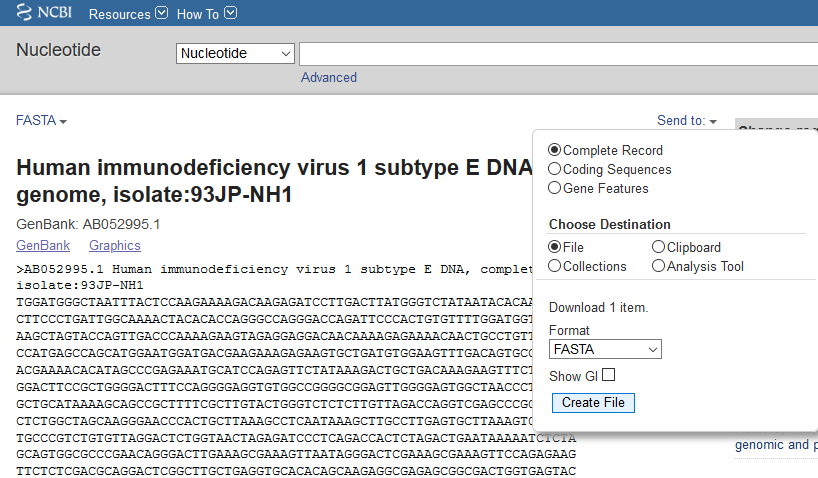
\includegraphics[scale=0.5]{ncbi3.png}
        \end{itemize}
    \end{frame}
    
    
    % cinomment out ko kasi meron naman explanation sa taas
    %\subsection{P2P Database}
    %\begin{frame}{P2P Databases}
    %    something explaining briefly p2p databases
    %\end{frame}
    
        \subsection{BioTorrents}
    \begin{frame}{P2P: BioTorrents}
        \begin{itemize}
            \item Scientific data continues to grow, and so does the demand for easier accessibility
            \item Centralized servers using HTTP or FTP cannot keep up with concurrent requests
            \item Peer-to-peer protocols does not scale well for large files
            \item BitTorrent handles both these problems
        \end{itemize}
    \end{frame}
    
    \begin{frame}{P2P: BioTorrents}
        \begin{itemize}
        \item System for legally sharing scientific data that works on top of the BitTorrent protocol. It is much like a public tracker.
        \item The main website hosts .torrent and metadata files
        \item Info about each dataset includes categories, license, filenames, etc. that helps users in searching for relevant datasets
        \item Torrent file has list of trackers, servers that "know" which peers are serving which files.
        \item Torrent client downloads from multiple peers simultaneously.
        \item To upload a torrent, the client makes a .torrent file using the torrenting software, then uploads it to the main website along with metadata. The client must have their computer continuously turned on to keep the file available as a peer. \cite{biotorrents}
        \end{itemize}
    \end{frame}
    
    \begin{frame}{P2P: BioTorrents}
        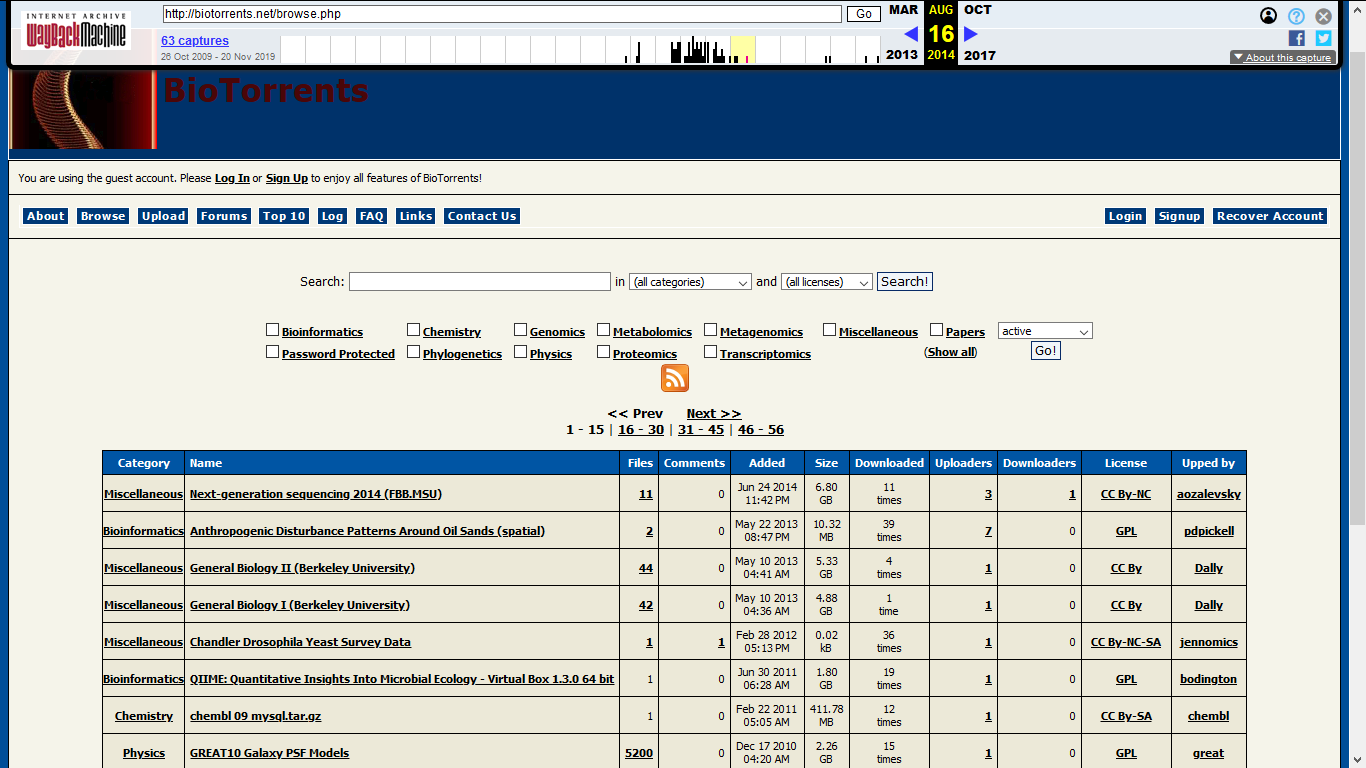
\includegraphics[scale=0.33]{biotorrents-page.png}
    \end{frame}
    
    \begin{frame}{P2P: BioTorrents}
        \begin{itemize}
            \item As with all public trackers, BioTorrents requires "good souls" that will keep many torrents available as often as possible.
            \item The datasets must be moderated to prevent abuse.
            \item The BioTorrents website is no longer up.
        \end{itemize}
    \end{frame}
 
    
    \subsection{PeerDB}
    \begin{frame}{P2P: PeerDB}
    % try adding screenshots
        \begin{itemize}
            \item Proposed P2P system for sharing general data
            \item Each node is equipped with a database
            \item Queries are passed around neighbors, with a maximum number of hops
            \item Caches information about other peers to speed up queries
            \item Large number of nodes \& relatively small number of lookup servers
            \cite{peerdb}
        \end{itemize}
    \end{frame}
    
    \subsection{Distributed Database}
    \begin{frame}{Distributed Databases}
        \begin{itemize}
            \item \textbf{Distributed Database}
            \begin{itemize}
                \item A distributed database system consists of loosely coupled sites that share no physical component             
                \item Database systems that run on each site are independent of each other
                \item Transactions may access data at one or more sites
                \cite[Ch.~19]{Silberschatz2010}
                \item Beneficial for large data with a certain speed requirement
            \end{itemize}
        \end{itemize}
    \end{frame}

        
    \subsection{SeqTorr}
    \begin{frame}{Distributed: SeqTorr}
    \textbf{SeqTorr} \cite{seqtorr}
    \begin{itemize}
        \item Standard genomics workflow consists of uploading and downloading data on an international database like NCBI.
        \item Having a distributed scalable local infrastructure to store genomic data instead of relying on NCBI would be beneficial since
        \begin{itemize}
            \item only certain sequences in NCBI are relevant to the institutions (e.g. Asian sequences are needed more than Caucasian ones)
            \item researchers within the country can share data with fast speeds
            \item institutions can share in the hosting of data
        \end{itemize}
    \end{itemize}
    \end{frame}
    \begin{frame}{Distributed: SeqTorr}
    \begin{itemize}
        \item Utilizes distributed database
        \item Master node
        \begin{itemize}
            \item containing metadata of all the sequences
            \item where user authentication is handled
        \end{itemize}
        \item Data node
        \begin{itemize}
            \item contain a portion of all the sequences
            \item needs to replicate a sequence \texttt{r} times before a sequence is considered available
            \item proximity of data nodes can increase download speed
        \end{itemize}
        \item Defined API Implementation
        \begin{itemize}
            \item POST
            \item GET
            \item PUT
            \item DELETE
        \end{itemize}

    \end{itemize}
    \end{frame}
    
    
    \begin{frame}{Distributed: SeqTorr}
    % have a unified way of discussing each database
    % what aspects of the database to discuss each
    % extra features will come after
        Problems: % have one for each database system
        \begin{itemize}
            \item program not currently available
            \begin{itemize}
                \item cannot measure any statistics on this
            \end{itemize}
        \end{itemize}
    \end{frame}
    
    \begin{frame}{Table}
% Bio-related -> biological
% What's the difference between biological vs general vs FASTA
% What does general mean?
% What does biological mean? -> explain pa to
% May 3 types of data ...
   \begin{table}[]
        \begin{tabular}{|l|l|l|l|l|}
        \hline
        System      & CS/P2P/H & Available? & DL/UL speed & Type of Data \\ \hline
        BioTorrents & P2P           & No         & Depends                    & Biological  \\ \hline
        SeqTorr     & H             & No         & Fast (PH server)           & FASTA        \\ \hline
        PeerDB      & P2P           & No         & Depends                    & General      \\ \hline
        NCBI        & CS            & Yes        & Slow (US server)           & Biological  \\ \hline
        \end{tabular}
    \end{table} 
\end{frame}

%%%%%%%%%%%%%%%%%%%%%%%%%%%%%%% PROBLEM %%%%%%%%%%%%%%%%%%%%%%%%%%%%%%%%%%%%

\section{Problem}
% after discussion of dist. databases
\begin{frame}{Problem}
The different gaps or problems found with other implementations
\textbf{Problems of Classical Databases}
\begin{enumerate}
%PROBLEMS OF CLASSICAL DATABASES (ALL FOUR)
    \item Genome researchers download entire database of genomic data
    \item Genome researchers only need a portion of the database, but end up downloading everything  (gigabytes size)
    \item Client-Server approach can face bottlenecks (server speed) %is resolved by making it more distributed
    \end{enumerate}
% or having a hard time getting a portion of the database
% easier to download parts vs whole, whole vs parts

% not easy to navigate the database? 
% what is the big problem? too big data to download all at once?
% why is it a problem? speed of download? or size?

\textbf{Problems of Distributed Databases}

\begin{enumerate}
%PROBLEM OF DIST. DATABASES
    \item Only one framework on distributed database for genomes
    \item Existing distributed database for genome code has little documentation % concept of APIs and documentation

\end{enumerate}
\end{frame}

%%%%%%%%%%%%%%%%%%%%%%%%%%%%% TITLE %%%%%%%%%%%%%%%%%%%%%%%%%%%%%%%%%%%%%%%%%%%%%%
\begin{frame}
\titlepage % Print the title page as the first slide
\end{frame}


%%%%%%%%%%%%%%%%%%%%%%%%%%%%%%%%%%%%% OBJECTIVES %%%%%%%%%%%%%%%%%%%%%%%%%%%%%%%%%%%%%%%%

\section{Objectives}
% to tackle those problems
% should be written in connection with the problems said:
% problem x : objective x
% para mas clear yung objectives

\begin{frame}{Objectives}
Based on the problems we found earlier, we propose the following objectives
 \begin{itemize}
    \item Create an information system that speeds up the download and upload of genomic data
    \begin{itemize}
        \item To resolve 1 \& 2 of the Problems of Classical Databases. 
    \end{itemize}
\end{itemize}

\begin{itemize}
    \item The system should have the main API’s
    \begin{itemize}
        \item POST genome data
        \item GET genome data (implement hybrid P2P)
        \begin{itemize}
            \item This will aim to resolve number 3 in the Problems of Classical Databases
        \end{itemize}
        \item PUT genome metadata (optional: PUT data)
        \item DELETE genome data
    \end{itemize}
    \item Write documentation for the system
    \begin{itemize}
        \item This will be used to resolve the Problems of Distributed Databases
    \end{itemize}
\end{itemize}
\end{frame}

\section{Scope}
\begin{frame}{Scope}
The current scope and coverage of the project is only
\begin{itemize}
    \item Security and Authentication is not part of the scope
    \item Use only FASTA file format 
    \begin{itemize}
        \item DNA nucleotides only
    \end{itemize}
    \item Only a proof of concept, UI will be purely for functional purposes (very basic design)
\end{itemize}
\end{frame}

%%%%%%%%%%%%%%%%%%%%%%%%%%%%%%%%%%%%%% THEORETICAL FRAMEWORK %%%%%%%%%%%%%%%%%%%%%%%%%%%%%%%%%%

\section{Theoretical Framework}

        \begin{frame}{Network Layers}

         \textbf{Networks Layers} how computers pass data to each other
        \begin{itemize}
            \item \begin{itemize}
            \item Level 1: Medium used to send signals (physical, electrical signals of 0 and 1), through wire or by air
            \item Level 2: Introduction of packets: Wifi, Ethernet, connecting together different . Goal of sending a group of signals.
            \item Level 3: Introduction of networks: IP Address to uniquely identify entities. 
            \item Level 4: Management of error free data transmission: Sending a group of messages via TCP, UDP, FTP
            \item \textbf{Level 5}: Abstraction of Level 4: Function calls programmers will use to do level 4 processes.
            \end{itemize}
        \end{itemize}
    \end{frame}
    
    \subsection{Application Architecture}
    % part ng theoretical framework
    % pwedeng walang slide of c/s
    % pwedeng ibanggit nalang ang client-server architecture

    % methods: ito framework
    % implemens client-server...
    \begin{frame}{Application Architecture}
        \begin{itemize}
            \item The \textbf{application architecture} is how a networked app is structured across the various end systems (i.e. computers, servers, etc.) \cite{kurose}
            \item Falls into either client-server, peer-to-peer, or hybrid architecture
        \end{itemize}
    \end{frame}
       
       
        \subsubsection{Client-Server}
        \begin{frame}{Client-Server}
            \begin{itemize}
                \item A \textbf{client-server} architecture relies on a Web server that is always available and has a fixed IP address\\
                \item A single server connects to many clients
            \end{itemize}
            \centering
            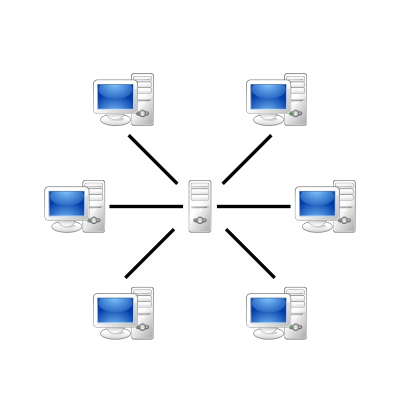
\includegraphics[scale=0.5]{Server-based-network.png}
        \end{frame}
       
       
        \subsubsection{Peer-to-Peer \& Hybrid}
        \begin{frame}{Peer-to-Peer \& Hybrid}
            \begin{itemize}
                \item A \textbf{peer-to-peer (P2P)} architecture has minimal to no reliance on always-on, dedicated servers
                \item Peers are desktops/laptops that communicate to each other without passing through a dedicated server
                \item A \textbf{hybrid} architecture combines elements of P2P and client-server architectures, attempting to utilize advantages of both
            \end{itemize}
            \centering
            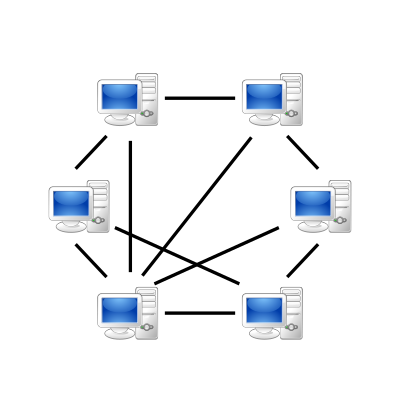
\includegraphics[scale=0.5]{P2P-network.png}
        \end{frame}
        
        \begin{frame}{Bittorent terminology}
            % ADD SCREENSHOT
            Peers \\ \\ 
             \centering
            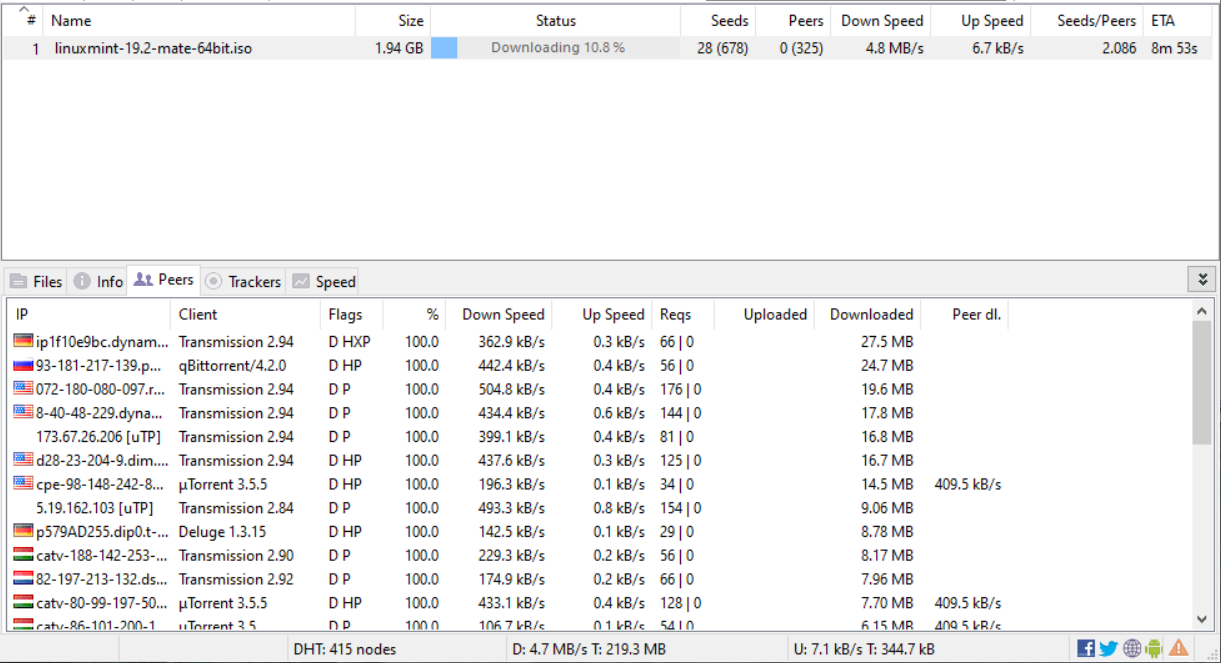
\includegraphics[scale=0.5]{bit-2.PNG}
        \end{frame}
        
        \begin{frame}{Bittorent terminology}
            % ADD SCREENSHOT
            Trackers \\ \\
             \centering
            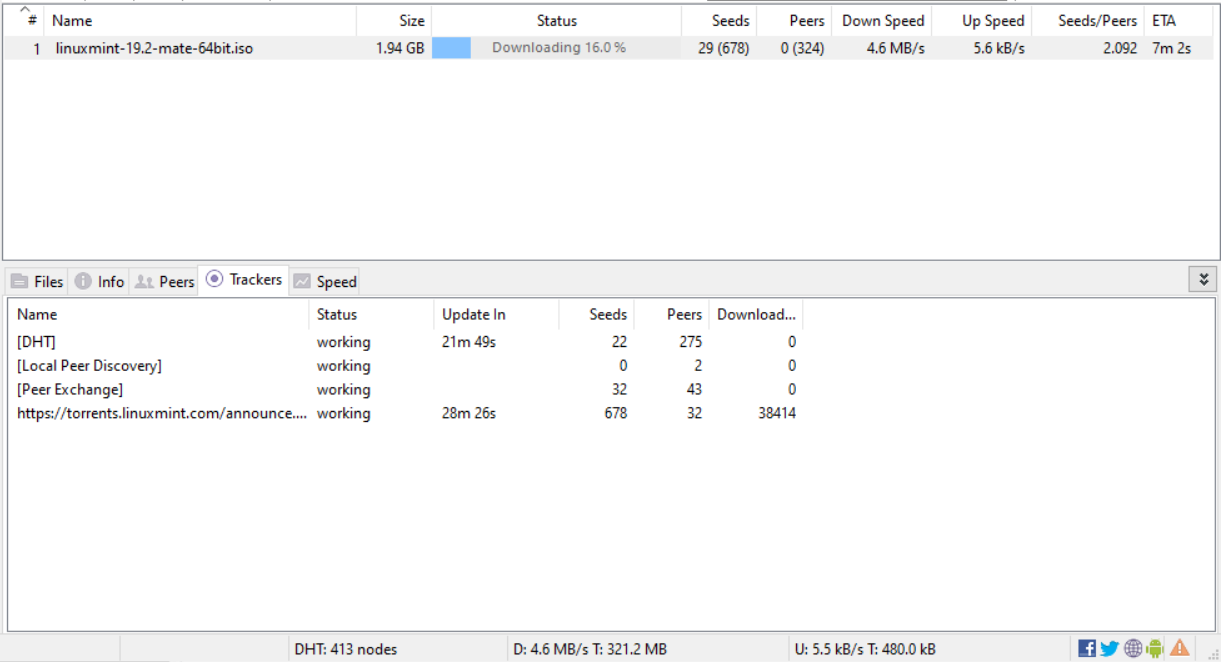
\includegraphics[scale=0.5]{bit-3.PNG}
        \end{frame}
        
        \begin{frame}{BitTorrent terminology}
            % visually show each term din
            % screenshot of torrent
            \begin{itemize} % siguro breeze through what these mean 
                \item \textbf{Peers} are users that connect to the BitTorrent network.
                \item \textbf{Torrent files} contain metadata about files \& folders, trackers, and hash values.
                \item \textbf{Trackers} are servers that keep track of peers and availability of files
                \item \textbf{Seeds} are peers which have downloaded the entire file and are making it available
            \end{itemize}
        \end{frame}




\begin{frame}{Theoretical Framework: System Description}
    \begin{itemize}
        \item A \textbf{master node} stores metadata of all sequences, may or may not contain sequence files
        \item \textbf{Data nodes} stores sequence files \& metadata of all sequence files in its filesystem
        \item Both master node \& data nodes have user interface that allow users to upload, search, and download sequence files
    \end{itemize}
\end{frame}

% DRAW.IO FILE: https://drive.google.com/file/d/1Nbp0Kmgcr2BZ13LBT3SGLMBoA6JA_Eth/view
\begin{frame}{Theoretical Framework: Schematics}
\textbf{App network diagram} \\ \medskip
\centering
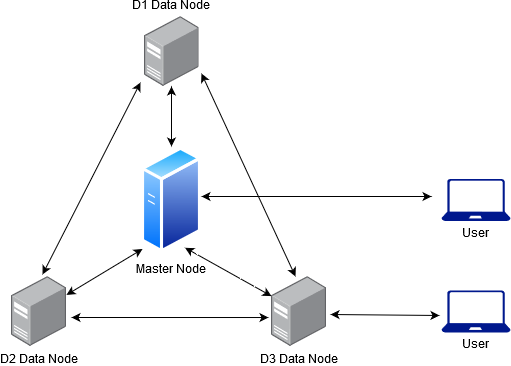
\includegraphics[scale=0.5]{thesis1.png}
\end{frame}

\begin{frame}{Theoretical Framework: Schematics}
\textbf{POST: Uploading a sequence to the master node} \\ \medskip
\centering
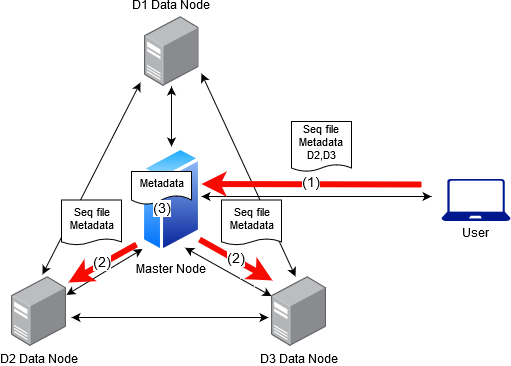
\includegraphics[scale=0.5]{thesis3.png}
\end{frame}

\begin{frame}{Theoretical Framework: Schematics}
\textbf{POST: Uploading a sequence to a data node} \\ \medskip
\centering
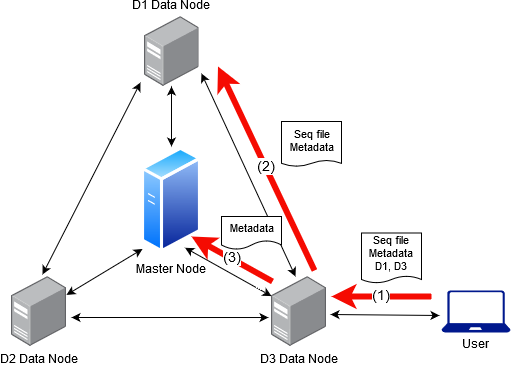
\includegraphics[scale=0.5]{thesis2.png}
\end{frame}

\begin{frame}{Theoretical Framework: Schematics}
\textbf{GET: Downloading a sequence} \\ \medskip
\centering
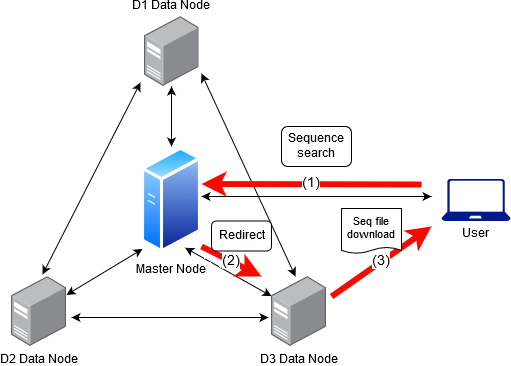
\includegraphics[scale=0.5]{thesis4.png}
\end{frame}

\subsection{Data Model}
\begin{frame}{Data Model}
This data model is lifted from SeqTorr \cite{seqtorr}


\small
\begin{center}
    

\begin{tabular}{c|c}
\hline
    key & description \\
\hline
\hline
    seq\textunderscore id & unique ID assigned to all sequences \\
    organism & organism where the sequence was extracted from \\
    quality & the rating of the data based on the number of downloads or another criteria \\
    uploader & user that uploaded the data \\
    institute & institute where the uploader or sequence was taken from \\
    upload\textunderscore date & date the data was uploaded to the database \\
    last\textunderscore modified & the date the metadata or data was edited \\
    data\textunderscore nodes & list of data nodes that this data contains
\end{tabular}
\end{center} 


\end{frame}

\subsection{Data Permissions}
\begin{frame}{Data Permissions}
\begin{center}
\begin{tabular}{c|c}
\hline
    user & description \\
\hline
\hline
   Moderator & Has ability to upload, download, store data, verify \\
    Peer & Has ability to upload, download, store data \\
    Guest & Has ability to upload, download \\

\end{tabular}
\end{center}

\end{frame}


\subsection{System Summary}
\begin{frame}{System}
  \begin{itemize}   
    \item system is this
    \item distributed
    \item community assisted
  \end{itemize}
\end{frame}

\begin{frame}{Summary}
  \begin{itemize}   
    \item 
    \item 
    \item 
  \end{itemize}
\end{frame}

\subsection{Community}
\begin{frame}{Community}
  \begin{itemize}   
    \item good for community
    \item easy to expand storage
    \item 
  \end{itemize}
\end{frame}

\subsection{Comparisons}
\begin{frame}{Speed Comparisons}
  \begin{itemize}   
    \item simple time complexity chart
    \item faster si caDDS ofc 
    \item 
  \end{itemize}
\end{frame}


\begin{frame}{Final Comparisons}
  \begin{itemize}   
    \item caDDS is scalable, easy for community, has docu hehe
    \item NCBI is one, stable, widely used
    \item 
  \end{itemize}
\end{frame}


\begin{frame}{Recommendations}
  \begin{itemize}   
    \item implement
    \item security
    \item public code
  \end{itemize}
\end{frame}

\begin{frame}
\Huge{\centerline{The End}}
\small{\centerline{Thank you for coming}}
\end{frame}

\section{Bibliography}

\begin{frame}[allowframebreaks]
\printbibliography[heading=none]
\end{frame}


\end{document}

